\documentclass[a4paper,12pt]{article}
\usepackage{xeCJK}          % 中文支持
\usepackage{fontspec}       % 英文/数学字体
\usepackage{amsmath, amssymb} % 数学公式
\usepackage{graphicx}       % 插入图片
\usepackage{hyperref}       % 目录超链接
\usepackage{geometry}       % 页面布局
\usepackage{bm}             % 粗体
\usepackage{xcolor}         % 颜色
\usepackage{tabularx}       % 表格环境
\usepackage{tikz}           % TikZ 绘制主对角线斜线
\usepackage{tcolorbox}
\geometry{left=3cm,right=3cm,top=3cm,bottom=3cm}

% 抽离颜色和尺寸参数
\newcommand{\analysisTitleColor}{green!50!black}
\newcommand{\analysisBackColor}{white}
\newcommand{\analysisBoxRule}{0.8pt}
\newcommand{\analysisArc}{3pt}
\newcommand{\analysisPadding}{6pt}

% 定义 tcolorbox
\newtcolorbox{analysisbox}{
    title=解析,
    colback=\analysisBackColor,
    colframe=\analysisTitleColor,
    boxrule=\analysisBoxRule,
    arc=\analysisArc,
    left=\analysisPadding,
    right=\analysisPadding,
    top=4pt,
    bottom=4pt
}

% =========================
% 字体设置
% =========================
\setmainfont{Times New Roman}
\setsansfont{Helvetica Neue}
\setmonofont{Menlo}
\setCJKmainfont{PingFang SC}

% =========================
% 图形路径(可调整)
% =========================
\graphicspath{{./assets/}}

% =========================
% 文档开始
% =========================
\begin{document}

%    \title{Template}
%    \author{Bowen}
%    \date{\today}
%    \maketitle

% =========================

    \section{线性方程组}

    \subsection{基础概念}

    \begin{enumerate}
        \item 方程组
        \[
            \begin{cases}
                a_{11}x_1 + a_{12}x_2 + \cdots + a_{1n}x_n = b_1 \\
                a_{21}x_1 + a_{22}x_2 + \cdots + a_{2n}x_n = b_2 \\
                \quad \vdots \\
                a_{m1}x_1 + a_{m2}x_2 + \cdots + a_{mn}x_n = b_m
            \end{cases}
        \]
        称为$n$个未知数$m$个方程的\textbf{非齐次线性方程组}。用矩阵表示为: $\mathbf{\color[rgb]{0.2, 0.6, 0.3}{Ax = b}}$其中$x = (x_1, x_2, \dots, x_n)^T, b = (b_1, b_2, \dots, b_n)^T$,
        \item 如果$b_{i} = 0(\forall i = 1,2,\dots,m)$,则称方程组
        \[
            \begin{cases}
                a_{11}x_1 + a_{12}x_2 + \cdots + a_{1n}x_n = 0 \\
                a_{21}x_1 + a_{22}x_2 + \cdots + a_{2n}x_n = 0 \\
                \quad \vdots \\
                a_{m1}x_1 + a_{m2}x_2 + \cdots + a_{mn}x_n = 0
            \end{cases}
        \]
        为\textbf{齐次线性方程组}
        \item 若用一组数$c_1, c_2, \dots, c_n$分别代替方程组中的$x_1, x_2, \dots, x_n$,使$m$个等式都成立,则称有序数组$(c_1, c_2, \dots, c_n)$是方程组的一组解。解方程组就是要找出方程组的全部解
        \item 非齐次线性方程组的全体系数及常数项所构成的矩阵
        \[
            \bar{A} =
            \begin{bmatrix}
                a_{11} & a_{12} & \dots  & a_{1n} & \;\big|\; & b_1    \\
                a_{21} & a_{22} & \dots  & a_{2n} & \;\big|\; & b_2    \\
                \vdots & \vdots & \ddots & \vdots & \;\big|\; & \vdots \\
                a_{m1} & a_{m2} & \dots  & a_{mn} & \;\big|\; & b_m
            \end{bmatrix}
        \]
        称为非齐次线性方程组的\textbf{增广矩阵},而由全体系数组成的矩阵
        \[
            A =
            \begin{bmatrix}
                a_{11} & a_{12} & \cdots & a_{1n} \\
                a_{21} & a_{22} & \cdots & a_{2n} \\
                \vdots & \vdots & \ddots & \vdots \\
                a_{m1} & a_{m2} & \cdots & a_{mn}
            \end{bmatrix}
        \]
        称为非齐次线性方程组的\textbf{系数矩阵}
        \item 如果两个方程组有相同的解集合,则称它们是\textbf{同解方程组}
        \item 下列三种变换称为线性方程组的\textbf{初等变换}
        \begin{enumerate}
            \item 用一个非零常数乘方程的两边
            \item 把某方程的$k$倍加到另一方程上
            \item 互换两个方程的位置
        \end{enumerate}
        线性方程组经初等变换华为阶梯形方程组后,每个方程中的第一个未知量\textbf{\color{red}{通常}}称为\textbf{主变量},其余的未知量称为\textbf{自由变量}
        \item 选择自由变量准则: \textbf{去掉自由变量后主变量行列式不能为0}
        \item 向量组$\eta_1, \eta_2, \dots, \eta_n$称为齐次线性方程组$Ax = 0$的\textbf{基础解系},如果
        \begin{enumerate}
            \item $\eta_1, \eta_2, \dots, \eta_n$是$Ax = 0$的解
            \item $\eta_1, \eta_2, \dots, \eta_n$线性无关
            \item $Ax = 0$的任一解都有由$\eta_1, \eta_2, \dots, \eta_n$线性表出
            \item 解向量个数
            \begin{align*}
                &= \; \text{无关解个数} \\
                &= \; \text{自由变量个数} \\
                &= \; t = n - r(A)\text{,其中}n = A\text{的列向量个数}
            \end{align*}
        \end{enumerate}
        \item 如果$\eta_1, \eta_2, \dots, \eta_n$是齐次线性方程组$Ax = 0$的一组基础解系,那么对任意常数$c_1, c_2, \dots, c_n$,
        \[
            c_{1}\eta_1 + c_{2}\eta_2 + \dots + c_{t}\eta_t
        \]
        是齐次线性方程组$Ax = 0$的\textbf{通解}
        \item $Ax = 0$\textbf{的基础解系是不唯一的}
        \item 对于方程组(I)和(II),如果$\alpha$既是方程组(I)的解,也是方程组(II)的解,则称$\alpha$是方程组(I)和(II)的\textbf{公共解}
        \item 对于方程组(I)和(II),如果$\alpha$是方程组(I)的解,则$\alpha$必是(II)的解;反过来,如果$\alpha$是方程组(II)的解,则$\alpha$必是(I)的解,则称(I)和(II)\textbf{同解}
        \item $Ax = 0$与$Bx = 0$同解
        \begin{align*}
            &\Leftrightarrow\; r(A) = r(B)\text{且}Ax = 0 \text{的解全是} Bx = 0\text{的解} \\
            &\Leftrightarrow\; r(A) = r(B) = r\!\left(\begin{bmatrix}
                                                          A \\ B
            \end{bmatrix}\right) \\
            &\Leftrightarrow\; \text{矩阵}A\text{和}B\text{的行向量组等价}
        \end{align*}
        \item 矩阵乘法一般没有交换律,若$AB = BA$,就称$A$与$B$\textbf{可交换}
    \end{enumerate}

    \subsection{定理}

    \begin{enumerate}
        \item 线性方程组的初等行变化把线性方程组变成与它同解的方程组
        \item 设$n$元非齐次线性方程组,对它的增广矩阵施行高斯消元法,得到阶梯形矩阵
        \[
            \bar A =
            \begin{bmatrix}
                c_{11} & c_{12} & \cdots & c_{1r} & \cdots & a_{1n} & d_1     \\
                & c_{22} & \cdots & c_{2r} & \cdots & a_{2n} & d_2     \\
                &        & \ddots & \vdots &        & \vdots & \vdots  \\
                &        &        & c_{rr} & \cdots & a_{rn} & d_r     \\
                &        &        & 0      & \cdots & 0      & d_{r+1} \\
                &        &        &        & \ddots & \vdots & \vdots  \\
                &        &        &        &        & 0      & 0       \\
            \end{bmatrix}.
        \]
        \begin{enumerate}
            \item 如果$d_{r+1} \neq 0$,方程组\textbf{无解}
            \item 如果$d_{r+1} = 0$,方程组\textbf{有解},并且
            \begin{enumerate}
                \item 当$r = n$时有唯一解
                \item 当$r < n$时有无穷多解
            \end{enumerate}
        \end{enumerate}
        \item 齐次线性方程组只有\textbf{零解(唯一解)}
        \begin{align*}
            &\Leftrightarrow\; r(A) = n  \\
        \end{align*}
        \item 齐次线性方程组有\textbf{非零解(有无穷多解)}
        \begin{align*}
            &\Leftrightarrow\; r(A) < n  \\
            &\Leftrightarrow\; A\text{的列向量线性无关} \\
            &\Leftrightarrow\; \text{若} m = n, \text{则} |A| = 0
        \end{align*}
        \item 当$m < n$(即方程的个数 < 未知数的个数)时,齐次线性方程组必有\textbf{非零解(有无穷多解)}
        \item 设齐次线性方程组系数矩阵的秩$r(A) = r < n$,则$Ax = 0$的基础解系由$n - r(A)$个线性无关的解向量所构成
        \item \textbf{有解判定定理}: 非齐次线性方程组 $\mathbf{\color[rgb]{0.2, 0.6, 0.3}{Ax = b}}$ 的解的充分必要条件是其系数矩阵和增广矩阵的秩相等,即 $\mathbf{r(A) = r(\overline{A})}$:
        \[
            \begin{aligned}
                & \text{若} r(A) = r(\bar{A}) = n && \Leftrightarrow \; \textbf{方程组有唯一解}  \\
                & \text{若} r(A) = r(\bar{A}) < n && \Leftrightarrow \; \textbf{方程组有无穷解}  \\
                & \textbf{方程组有解} &&
                \begin{cases}
                    \Leftrightarrow r(A) = r(\bar{A}) \\
                    \Leftrightarrow A \text{的行向量组线性无关} \\
                    \text{原因:}r(A) \le r(\bar{A}) \le m \Rightarrow r(A) = r(\bar{A}) = m
                \end{cases} \\
                & \text{非齐次线性方程组} \mathbf{\color[rgb]{0.2, 0.6, 0.3}{Ax = b}} \text{无解} &&
                \begin{cases}
                    \Leftrightarrow \mathbf{r(A) + 1 = r(\overline{A})} \\
                    \Leftrightarrow b \text{不能由} A \text{的列向量线性表出} \\
                    \Rightarrow |A| = 0
                \end{cases}
            \end{aligned}
        \]
        \item \textbf{解的性质}
        \begin{enumerate}
            \item 如果$\eta_1, \eta_2$是齐次线性方程组$Ax = 0$的两个解,那么其线性组合仍是该齐次线性方程组$Ax = 0$的解
            \item 如果$\alpha, \beta$是非齐次线性方程组$\mathbf{\color[rgb]{0.2, 0.6, 0.3}{Ax = b}}$的两个解,则$\alpha - \beta$是导出组$Ax = 0$的解
            \begin{align*}
                &\Leftrightarrow\; r(A) = r(\overline{A}) < n  \\
                &\Leftrightarrow\; Ax = 0\text{有无穷多解}
            \end{align*}
            \item 如果$\alpha$是齐次线性方程组$\mathbf{\color[rgb]{0.2, 0.6, 0.3}{Ax = b}}$的解,$\eta$是导出组$Ax = 0$的解,则$\alpha + \eta$是非齐次线性方程组$\mathbf{\color[rgb]{0.2, 0.6, 0.3}{Ax = b}}$的解
            \item 使用 \textbf{\color{red}{最小公约数}} 构造解:
            \[
                \alpha_1 + \alpha_2 \quad \text{是两个解,} \quad
                \alpha_2 + 2\alpha_3 \quad \text{是三个解,}
            \]
            故可构造:
            \[
                3(\alpha_1 + \alpha_2) - 2(\alpha_2 + 2\alpha_3)
            \]
            \item 若$\alpha_1,\alpha_2,\dots,\alpha_t$是$\mathbf{\color[rgb]{0.2, 0.6, 0.3}{Ax = b}}$的解
            \begin{enumerate}
                \item 且$k_1 + k_2 + \dots + k_t = 1$ \Leftrightarrow $k_{1}\alpha_1 + k_{2}\alpha_2 + \dots + k_{t}\alpha_t$仍是$Ax = \mathbf{b}$的解
                \item 且$k_1 + k_2 + \dots + k_t = 0$ \Leftrightarrow $k_{1}\alpha_1 + k_{2}\alpha_2 + \dots + k_{t}\alpha_t$仍是$Ax = \mathbf{0}$的解
            \end{enumerate}
        \end{enumerate}
        \item \textbf{解的结构}: 对非齐次线性方程组$\mathbf{\color[rgb]{0.2, 0.6, 0.3}{Ax = b}}$,若$r(A) = r(\bar{A}) = r$,且已知$\eta_1, \eta_2, \dots, \eta_{n - r}$是导出组$Ax = 0$的基础解系,$\zeta_0$是$\mathbf{\color[rgb]{0.2, 0.6, 0.3}{Ax = b}}$的每个已知解,则$\mathbf{\color[rgb]{0.2, 0.6, 0.3}{Ax = b}}$的通解为
        \[
            \zeta_0 + c_{1}\eta_1 + c_{2}\eta_2 + \dots + c_{n-r}\eta_{n-r}
        \]其中$c_1, c_2, \dots, c_{n-r}$为任意常数
        \item 通解表示为:
        \[
            \begin{aligned}
                \text{通解}
                &= \text{特解} + k_1 \text{解向量}_1 + k_2 \text{解向量}_2 + \dots \\
                &= \text{特解} + \text{齐次方程 } Ax = 0 \text{ 的通解}
            \end{aligned}
        \]

        特解构造方法:
        \[
            \begin{aligned}
                \text{特解} &= \text{令自由变量为0,主元为常数项} \\
                \text{特解} &\Leftarrow \text{通过单个 } b \text{ 构造,即除/减 } (n+1 \text{ 个解 } - n \text{ 个解})
            \end{aligned}
        \]

        齐次方程 $Ax = 0$ 的通解:
        \[
            \begin{aligned}
                \text{通解} &= \text{自由变量列的相反数} \\
                \text{通解} &= \alpha - \beta \; \text{或通过 {\color{red}{最小公倍数}} 法构造}
            \end{aligned}
        \]
    \end{enumerate}

    \subsection{运算}

    \begin{enumerate}

    \end{enumerate}

    \subsection{公式}

    \subsection{方法步骤}

    \begin{enumerate}
        \item $\mathbf{\color[rgb]{0.2, 0.6, 0.3}{Ax = b}}$ 有解 $\Leftrightarrow r(A) = r(\bar{A})$
        \begin{enumerate}
            \item 判断何时$a = 0$
            \[
                \bar{A} =
                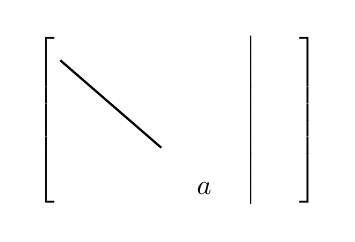
\begin{tikzpicture}[baseline=(current bounding box.center)]
                    % 放置矩阵
                    \node (mat) {
                        $\begin{bmatrix}
                             \; & \; & \; & \; & \; & \;\big|\; & \; \\
                             \; & \; & \; & \; & \; & \;\big|\; & \; \\
                             \; & \; & \; & \; & \; & \;\big|\; & \; \\
                             \; & \; & \; & \; & \; & \;\big|\; & \; \\
                             \; & \; & \; & \; & a  & \;\big|\; &
                        \end{bmatrix}$
                    };

                    % 画主对角线
                    % 从矩阵左上角到右下角(倒数第二列)
                    \draw[thick,black]
                    ([xshift=12pt,yshift=-12pt]mat.north west) --
                    ([xshift=-60pt,yshift=24pt]mat.south east);
                \end{tikzpicture}
            \]
            若$a = 0$则{\color{red}{有可能}}无解
            \begin{enumerate}
                \item $\forall a$均有解
                \[
                    \bar{A} =
                    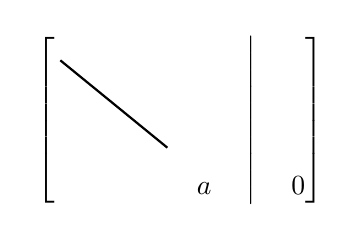
\begin{tikzpicture}[baseline=(current bounding box.center)]
                        % 放置矩阵
                        \node (mat) {
                            $\begin{bmatrix}
                                 \; & \; & \; & \; & \; & \;\big|\; & \; \\
                                 \; & \; & \; & \; & \; & \;\big|\; & \; \\
                                 \; & \; & \; & \; & \; & \;\big|\; & \; \\
                                 \; & \; & \; & \; & \; & \;\big|\; & \; \\
                                 \; & \; & \; & \; & a  & \;\big|\; & 0
                            \end{bmatrix}$
                        };

                        % 画主对角线
                        % 从矩阵左上角到右下角(倒数第二列)
                        \draw[thick,black]
                        ([xshift=12pt,yshift=-12pt]mat.north west) --
                        ([xshift=-60pt,yshift=24pt]mat.south east);
                    \end{tikzpicture}
                \] \\
                \item 若$b \neq 0$必无解
                \[
                    \bar{A} =
                    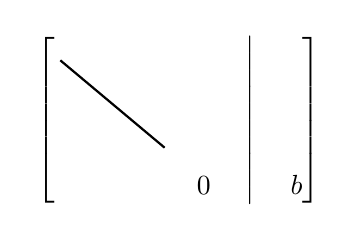
\begin{tikzpicture}[baseline=(current bounding box.center)]
                        % 放置矩阵
                        \node (mat) {
                            $\begin{bmatrix}
                                 \; & \; & \; & \; & \; & \;\big|\; & \; \\
                                 \; & \; & \; & \; & \; & \;\big|\; & \; \\
                                 \; & \; & \; & \; & \; & \;\big|\; & \; \\
                                 \; & \; & \; & \; & \; & \;\big|\; & \; \\
                                 \; & \; & \; & \; & 0  & \;\big|\; & b
                            \end{bmatrix}$
                        };

                        % 画主对角线
                        % 从矩阵左上角到右下角(倒数第二列)
                        \draw[thick,black]
                        ([xshift=12pt,yshift=-12pt]mat.north west) --
                        ([xshift=-60pt,yshift=24pt]mat.south east);
                    \end{tikzpicture}
                \]
            \end{enumerate}
            \item Case:
            \[
                \left[
                    \begin{array}{ccc|c}
                        1 & -1              & a                & 2   \\
                        & \underline{a-1} & a+2              & -3  \\
                        &                 & \underline{2a+6} & a-9
                    \end{array}
                    \right]
            \]
            从下向上依次检查与$0$的关系
            \begin{enumerate}
                \item 先看$2a + 6 = 0$
                \item 再看$a - 1 = 0$
            \end{enumerate}
            \begin{align*}
                & \text{唯一解} && \Leftrightarrow r(A) = r(\bar{A}) = n && \Leftrightarrow a \neq 1 \text{ 且 } a \neq -3 \\
                & \text{无穷解} && \Leftrightarrow r(A) = r(\bar{A}) < n && \Leftrightarrow a = 1 \\
                & \text{无解}   && \Leftrightarrow r(A) + 1 = r(\bar{A}) && \Leftrightarrow a = -3
            \end{align*}
        \end{enumerate}
        \item 证明$\alpha_1,\alpha_2,\dots,\alpha_t$是$Ax = 0$的基础解系,需要
        \begin{enumerate}
            \item 验证$\alpha_1,\alpha_2,\dots,\alpha_t$是$Ax = 0$的解
            \item 证明$\alpha_1,\alpha_2,\dots,\alpha_t$线性无关
            \item $t = n - r(A)$
        \end{enumerate}
        \item 非齐次线性方程组求解方法
        \begin{enumerate}
            \item 对增广矩阵作初等{\color{red}{行变换}}化为阶梯形矩阵
            \item 求导出组的几个基础解系
            \item 求方程组的一个特解(为简捷,可令自由变量全为0)
            \item 按解的结构写出通解
            \item 注: \textbf{当方程组中含有参数时,分析讨论要严谨不要丢情况}
        \end{enumerate}
        \item 公共解处理方法(例4.16)
        \begin{enumerate}
            \item (I)(II)联立求解
            \item 通过(I)与(II)各自的通解,寻找非零公共解
            \item 把(I)的通解带入(II)中,如果仍是解,寻找$k_1, k_2$所对应满足的关系式而求出公共解
        \end{enumerate}
        \item 证明两方程同解
        \begin{enumerate}
            \item 定义
            \item $r(A) = r(B)$且$Ax = 0$ 的解全是 $Bx = 0$的解
        \end{enumerate}
    \end{enumerate}

    \subsection{条件转换思路}
    \begin{enumerate}
        \item 抽象方程组(例4.9)
        \begin{enumerate}
            \item 解的结构
            \item 解的性质
            \item 秩
        \end{enumerate}
    \end{enumerate}

\end{document}
